% This is text associated with the open textbook "Open Electromagnetics"
% See immediately below for author, date
% This work is licensed under the Creative Commons Attribution-ShareAlike 4.0 International License. (CC BY-SA 4.0) 
% To view a copy of the license, visit http://creativecommons.org/licenses/by-sa/4.0/

%ORB TITLE Boundary Conditions on the Electric Field Intensity (${\bf E}$)
%ORB AUTHOR 0        # S.W. Ellingson, Virginia Tech (ellingson@vt.edu)
%ORB DATE 20180806   # yyyymmdd
%ORB ABSTRACT Boundary Conditions on the Electric Field Intensity 

\label{m0020_Boundary_Conditions_on_E} % <-- Must match name of this file and module directory name.  Don't mess with this!

In homogeneous media, electromagnetic quantities vary smoothly and continuously.
At an interface between dissimilar media, however, it is possible for electromagnetic quantities to be discontinuous.
These discontinuities can be described mathematically as \emph{boundary conditions} and used to to constrain solutions for the associated electromagnetic quantities.
In this section, we derive boundary conditions 
\index{boundary conditions}
on the electric field intensity ${\bf E}$.
\index{electric field intensity!boundary conditions}

To begin, consider a region consisting of only two media that meet at an interface defined by the mathematical surface ${\mathcal S}$, as shown in Figure~\ref{m0020_fPEC}.
%
\begin{figure}[b!]
\begin{center}
\pdftooltip{{  % note double braces
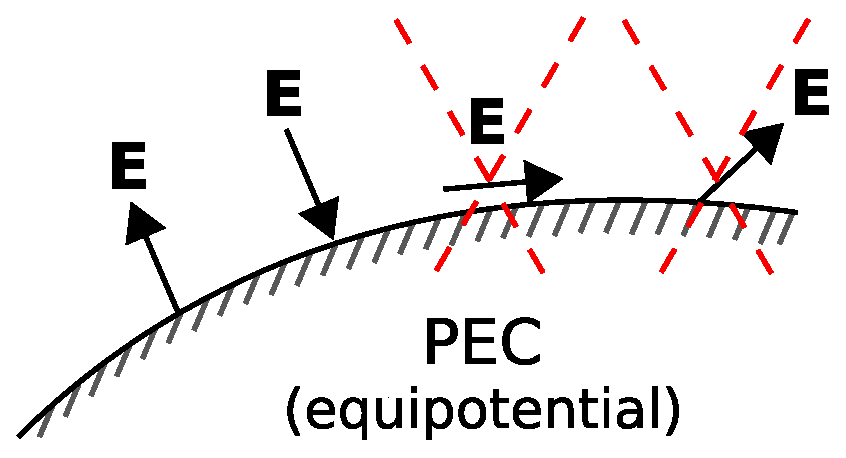
\includegraphics[width=2in]{modules/m0020_fPEC.eps}
% https://commons.wikimedia.org/wiki/File:M0020_fPEC.svg
}}{A curved, arbitrary surface labeled “PEC (equipotential)” shows four vectors labeled E. The leftmost vector is pointed away from the curved surface. The second vector is pointed toward the surface exactly opposite of the leftmost arrow. The third vector is tangent to the surface, pointing to the right, with a dashed red X over it. The fourth vector is at an acute angle to the surface, pointed diagonally to the upper right, with a dashed red X over it. }
\end{center} 
\centerline{\scriptsize 
\copyright~\hyperref[m0020_fPEC_Credit]{K.\ Kikkeri} 
\href{https://creativecommons.org/licenses/by-sa/4.0/}{CC BY~SA 4.0} 
} 
\caption{
\label{m0020_fPEC}
At the surface of a perfectly-conducting region, ${\bf E}$ may be perpendicular to the surface (two leftmost possibilities), but may not exhibit a component that is tangent to the surface (two rightmost possibilities).
}
\end{figure}
%
If either one of the materials is a perfect electrical conductor (PEC), 
\index{conductor!perfect}
then ${\mathcal S}$ is an equipotential surface; i.e., the electric potential $V$ is constant everywhere on ${\mathcal S}$.  
Since ${\bf E}$ is proportional to the spatial rate of change of potential (recall ${\bf E}=-\nabla V$; Section~\ref{m0063_Electric_Field_as_the_Gradient_of_Potential}), we find:
%
%ORB HIGHLIGHT
\begin{mdframed}[backgroundcolor=yellow!20,nobreak=true] 
The component of ${\bf E}$ that is tangent to a perfectly-conducting surface is zero.
\end{mdframed}
%
This is sometimes expressed informally as follows:
%
\begin{equation}
\boxed{
E_{tan} = 0~~\mbox{on PEC surface}
}
\end{equation}
%
where ``$E_{tan}$'' is understood to be the component of ${\bf E}$ that is tangent to ${\mathcal S}$. 
Since the tangential component of ${\bf E}$ on the surface of a perfect conductor is zero, the electric field at the surface must be oriented entirely in the  
direction perpendicular to the surface, as shown in Figure~\ref{m0020_fPEC}.

The following equation expresses precisely the same idea, but includes the calculation of the tangential component as part of the statement:
%
\begin{equation}
{\bf E} \times \hat{\bf n} = 0~~\mbox{(on PEC surface)}
\label{m0020_eEPECBC}
\end{equation} 
%
where $\hat{\bf n}$ is either normal (i.e., unit vector perpendicular to the surface) to each point on ${\mathcal S}$.
This expression works because the cross product of any two vectors is perpendicular to either vector (Section~\ref{m0006_Vector_Arithmetic}), and any vector which is perpendicular to $\hat{\bf n}$ is tangent to ${\mathcal S}$.

We now determine a more general boundary condition that applies even when neither of the media bordering ${\mathcal S}$ is a perfect conductor.
The desired boundary condition can be obtained directly from Kirchoff's Voltage Law (KVL; Section~\ref{m0016_Kirchoffs_Voltage_Law_Electrostatics_Integral_Form}):
\index{Kirchoff's voltage law!electrostatics}
% 
\begin{equation}  
\oint_{\mathcal{C}}{ {\bf E} \cdot d{\bf l} } = 0
\label{m0020_eKVL}
\end{equation}
% 
Let the closed path of integration take the form of a rectangle centered on ${\mathcal S}$, as shown in Figure~\ref{m0020_fKVL}.
%
\begin{figure}
\begin{center}
\pdftooltip{{  % note double braces
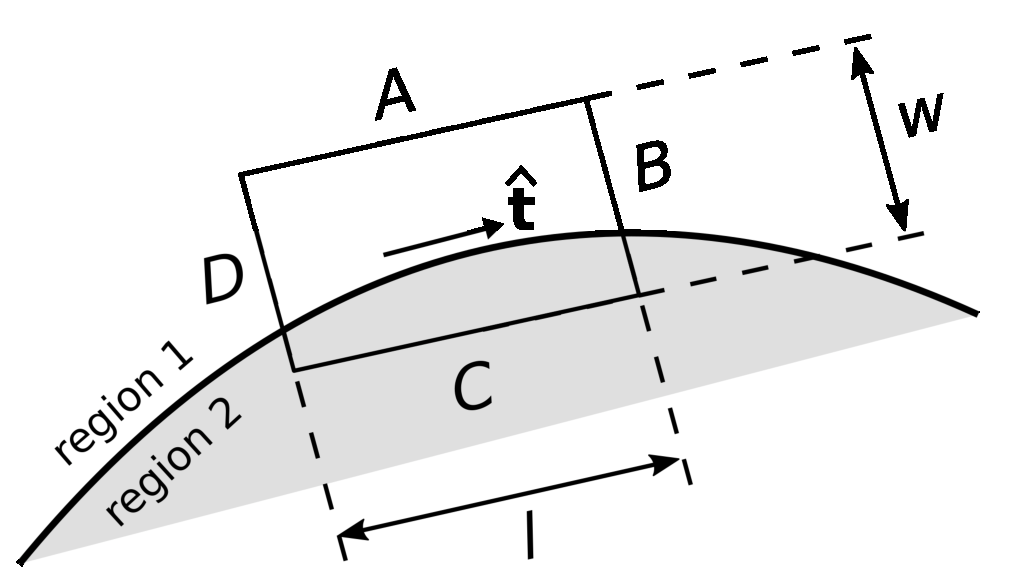
\includegraphics[width=2.5in]{modules/m0020_fKVL.eps}
% https://commons.wikimedia.org/wiki/File:M0020_fKVL.svg
}}{The figure shows a curved arbitrary surface labeled "C", the outside area labeled "region 1" and the inside, greyed area labeled "region 2". A vector tangent to the surface labeled t-hat is pointed to the right. A rectangle is shown surrounding the arrow. Starting with the top side and following a clockwise direction, the rectangle is labeled A, B, C, and D, with A and C being the longer sides. Dashed lines extend on side C with an arrow in between labeled, l. Dashed lines extend on side B with an arrow in between labeled w.}
\end{center} 
\centerline{\scriptsize 
\copyright~\hyperref[m0020_fKVL_Credit]{K.\ Kikkeri} 
\href{https://creativecommons.org/licenses/by-sa/4.0/}{CC BY~SA 4.0} 
} 
\caption{
\label{m0020_fKVL}
Use of KVL to determine the boundary condition on ${\bf E}$.
}
\end{figure}
%
Let the sides $A$, $B$, $C$, and $D$ be perpendicular or parallel to the surface, respectively.  
Let the length of the perpendicular sides be $w$, and let the length of the parallel sides be $l$.  
From KVL we have
% 
\begin{align}   
\oint_{\mathcal{C}}{ {\bf E} \cdot d{\bf l} } &= \int_A{ {\bf E} \cdot d{\bf l} } & \nonumber \\ 
                                &+\int_B{ {\bf E} \cdot d{\bf l} }  & \nonumber \\ 
                                &+\int_C{ {\bf E} \cdot d{\bf l} }  & \nonumber \\
                                &+\int_D{ {\bf E} \cdot d{\bf l} }  &= 0 
\end{align}
%  
Now, let us reduce $w$ and $l$ together while (1) maintaining a constant ratio $w/l\ll 1$ and (2) keeping $\mathcal{C}$ centered on $\mathcal{S}$.
In this process, the contributions from the $B$ and $D$ segments become equal in magnitude but opposite in sign; i.e., 
% 
\begin{equation}   
\int_B{ {\bf E} \cdot d{\bf l} } 
+\int_D{ {\bf E} \cdot d{\bf l} }
\to 0
\end{equation}
%
This leaves
% 
\begin{equation}   
\oint_{\mathcal{C}}{ {\bf E} \cdot d{\bf l} } \to \int_A{ {\bf E} \cdot d{\bf l} }+\int_C{ {\bf E} \cdot d{\bf l} }  \to 0 
\end{equation}
%
Let us define the unit vector $\hat{\bf t}$ (``tangent'') as shown in Figure~\ref{m0020_fKVL}.
When the lengths of sides $A$ and $C$ become sufficiently small, we can write the above expression as follows:
% 
\begin{equation}   
  {\bf E}_1 \cdot \hat{\bf t}\Delta l
- {\bf E}_2 \cdot \hat{\bf t}\Delta l 
\to 0
\label{m0020_eKVL2}
\end{equation}
%
where ${\bf E}_1$ and ${\bf E}_2$ are the fields evaluated on the two sides of the boundary and
$\Delta l\to 0$ is the length of sides $A$ and $C$ while this is happening.
Note that the only way Equation~\ref{m0020_eKVL2} can be true is if the tangential components of ${\bf E}_1$ and ${\bf E}_2$ are equal. In other words: 
%
%ORB HIGHLIGHT
\begin{mdframed}[backgroundcolor=yellow!20,nobreak=true] 
The tangential component of ${\bf E}$ must be continuous across an interface between dissimilar media. 
\end{mdframed}
%
Note that this is a generalization of the result we obtained earlier for the case in which one of the media was a PEC -- in that case, the tangent component of ${\bf E}$ on the other side of the interface must be zero because it is zero in the PEC medium.

As before, we can express this idea in compact mathematical notation.
Using the same idea used to obtain Equation~\ref{m0020_eEPECBC}, we have found
%
\begin{equation}
{\bf E}_1 \times \hat{\bf n} = {\bf E}_2 \times \hat{\bf n}~~~\mbox{on $\mathcal{S}$}
\end{equation}
%
or, as it is more commonly written:
%
\begin{equation}
\boxed{
\hat{\bf n} \times \left( {\bf E}_1 - {\bf E}_2 \right) = 0~~~\mbox{on $\mathcal{S}$}
}
\label{m0020_eBCE}
\end{equation} 

We conclude this section with a note about the broader applicability of this boundary condition:
%
%ORB HIGHLIGHT
\begin{mdframed}[backgroundcolor=yellow!20,nobreak=true] 
Equation~\ref{m0020_eBCE} is the boundary condition that applies to ${\bf E}$ for both the electrostatic \emph{and the general (time-varying) case.}
\end{mdframed}
%
Although a complete explanation is not possible without the use of the Maxwell-Faraday Equation (Section~\ref{m0050_Maxwell-Faraday_Equation}), the reason why this boundary condition applies in the time-varying case can be disclosed here.
In the presence of time-varying magnetic fields, the right-hand side of Equation~\ref{m0020_eKVL} may become non-zero and is proportional to the area defined by the closed loop. 
However, the above derivation requires the area of this loop to approach zero, in which case the possible difference from Equation~\ref{m0020_eKVL} also converges to zero.
Therefore, the boundary condition expressed in Equation~\ref{m0020_eBCE} applies generally.


